\section{Arrays}
\label{sec:arry}
\begin{frame}<beamer>
    \frametitle{Outline}
    \tableofcontents[currentsection]
\end{frame}

\begin{frame}[fragile]{Opening Discussion (1)}

\begin{itemize}
	\item {Given we have following problem}
	\begin{itemize}
		\item {We have 10 students in the class}
		\item {We want to get average/sum/max/min score of their math course}
		\item {We also want to rank the scores}
		\item {Based on what we learned}
		\item {We should keep 10 variables of the same type}
	\end{itemize}
	\item {How about we have 100 students??}
\end{itemize}
\vspace{-0.10in}
\begin{columns}
\begin{column}{0.75\linewidth}
\begin{lstlisting}
#include <stdio.h>
void main()
{
   float x1, x2, x3, x4, x5, x6,x7,x8,x9,x10;
   float sum = 0, avg = 0;
   scanf("%f", &x1);
   sum += x1;
   scanf("%f", &x2);
   sum += x2;
   ...
   avg = sum/10;
}
\end{lstlisting}
\end{column}
\end{columns}
\end{frame}

\begin{frame}[fragile]{Opening Discussion (2)}
\vspace{-0.15in}
\begin{columns}
\begin{column}{0.75\linewidth}
\begin{lstlisting}
#include <stdio.h>
void main()
{
   float x1, x2, x3, x4, x5, x6,x7,x8,x9,x10;
   float sum = 0, avg = 0;
   scanf("%f", &x1);
   sum += x1;
   scanf("%f", &x2);
   sum += x2;
   ...
   avg = sum/10;
}

\end{lstlisting}
\end{column}
\end{columns}
\vspace{-0.15in}
\begin{itemize}
	\item {Even that it is hard to do sorting}
	\begin{itemize}
		\item {Try your best to figure out how you can put fourty variables in order}
	\end{itemize}
	\item {This is where the \textcolor{red}{array} comes}
\end{itemize}

\end{frame}

\subsection{1D Array}
\label{sec:1darry}
\begin{frame}<beamer>
    \frametitle{Outline}
    \tableofcontents[currentsection, currentsubsection]
\end{frame}

\begin{frame}[fragile]{1D Array: declaration (1)}
\begin{itemize}
	\item {1D array is defined in following form}
\end{itemize}
\begin{center}
 \LARGE{
	\textcolor{blue}{type} \textcolor{red}{arrayName}[\textbf{size}];
	}
\end{center}
\begin{itemize}
	\item {\textcolor{blue}{type} could be any type defined in C, e.g. \textcolor{blue}{int}, \textcolor{blue}{float},...}
	\item {``\textcolor{red}{arrayName}'' should be \textcolor{red}{unique}}
	\item {It is actually a variable/constant, so rules to other variables/constants apply too}
	\item {``\textbf{size}'' should be an integer or an integer constant \textcolor{red}{greater than 0}}
\end{itemize}
\begin{lstlisting}[xleftmargin=0.09\linewidth, linewidth=0.9\linewidth, frame=no, numbers=none]
int a[0]; //it is grammar OK, but meaningless
\end{lstlisting}
\end{frame}

\begin{frame}[fragile]{1D Array: declaration (2)}
\begin{center}
 \LARGE{
	\textcolor{blue}{type} \textcolor{red}{arrayName}[\textbf{size}];
	}
\end{center}
\begin{itemize}
	\item {\textcolor{blue}{type} could be any type defined in C, e.g. \textcolor{blue}{int}, \textcolor{blue}{float},...}
	\item {``\textcolor{red}{arrayName}'' should be \textcolor{red}{unique}}
	\item {It is actually a variable/constant, so rules to other variables/constants apply too}
	\item {``\textbf{size}'' should be an integer or an integer constant \textcolor{red}{greater than 0}}
\end{itemize}
\begin{columns}
\begin{column}{0.25\linewidth}
\begin{lstlisting}
int main()
{
   float x[40];
   ....
   return 0;
}

\end{lstlisting}
\end{column}
\begin{column}{0.35\linewidth}
\begin{lstlisting}
int main()
{
   const int N = 40;
   float x[N];
   ....
   return 0;
}

\end{lstlisting}
\end{column}
\begin{column}{0.3\linewidth}
\begin{lstlisting}
int main()
{
   int N = 40;
   float x[N];
   ....
   return 0;
}

\end{lstlisting}
\end{column}
\end{columns}
\end{frame}

\begin{frame}[fragile]{1D Array: declaration (3)}
\begin{center}
 \LARGE{
	\textcolor{blue}{type} \textcolor{red}{arrayName}[\textbf{size}];
	}
\end{center}
\begin{itemize}
	\item {\textcolor{blue}{type} could be any type defined in C, e.g. \textcolor{blue}{int}, \textcolor{blue}{float},...}
	\item {``\textcolor{red}{arrayName}'' should be \textcolor{red}{unique}}
	\item {It is actually a variable/constant, so rules to other variables/constants apply too}
	\item {``\textbf{size}'' should be an integer or an integer constant \textcolor{red}{greater than 0}}
\end{itemize}
\begin{columns}
\begin{column}{0.25\linewidth}
\begin{lstlisting}
#define N 40
int main()
{
   float x[N];
   ....
   return 0;
}

\end{lstlisting}
\end{column}
\begin{column}{0.35\linewidth}
\begin{lstlisting}
int main()
{
   const int N = 40;
   float x[N];
   ....
   return 0;
}

\end{lstlisting}
\end{column}
\begin{column}{0.3\linewidth}
\begin{lstlisting}
#define N 40
int main()
{
   float x[3*N];
   ....
   return 0;
}

\end{lstlisting}
\end{column}
\end{columns}
\end{frame}

\begin{frame}[fragile]{1D Array: visit array element (1)}
\begin{itemize}
	\item {Element in an array is visited by the \textbf{subscript}}
	\item {Subscript starts from `\textcolor{green}{0}' to `\textcolor{green}{N-1}'}
	\item {For example, visit the 3rd element of x[N], we write ``x[2]''}
\end{itemize}
\begin{columns}
\begin{column}{0.2\linewidth}
\end{column}
\begin{column}{0.5\linewidth}
\begin{lstlisting}
#include <stdio.h>
int main()
{
   float x[40];
   x[0] = 5.0;
   x[2] = 3.1;
   printf("x[0] = %f", x[0]);
   return 0;
}

\end{lstlisting}
\end{column}
\begin{column}{0.2\linewidth}
\end{column}
\end{columns}
\end{frame}

\begin{frame}[fragile]{1D Array: visit array element (2)}
\begin{columns}
\begin{column}{0.2\linewidth}
\end{column}
\begin{column}{0.52\linewidth}
\begin{lstlisting}
int main()
{
   float x[40];
   int i = 0;
   for(i = 0; i < 40; i++)
   {
      printf("Input %d:", i);
      /*--be careful below--*/
      scanf("%f", &(x[i])); 
   }
   return 0;
}
\end{lstlisting}
\end{column}
\begin{column}{0.2\linewidth}
\end{column}
\end{columns}
\begin{itemize}
	\item {You are not allowed to use subscript beyond \textcolor{red}{39}}
	\item {You invade other's territory!!}
\end{itemize}
\end{frame}

\begin{frame}[fragile]{1D Array: how array looks like (1)}
\begin{columns}
\begin{column}{0.5\linewidth}
\begin{figure}
	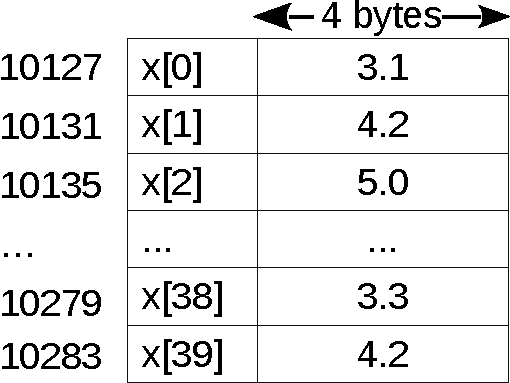
\includegraphics[width=0.88\linewidth]{figs/farray.pdf}
\end{figure}
\end{column}
\begin{column}{0.5\linewidth}
\begin{figure}
	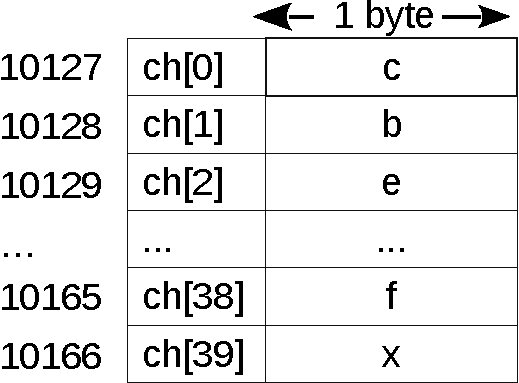
\includegraphics[width=0.9\linewidth]{figs/charray.pdf}
\end{figure}
\end{column}
\end{columns}
\vspace{0.1in}
\begin{itemize}
	\item {The system opens a continuous memory block for an array}
	\item {Actual size depends on both the type and length of an array}
\end{itemize}
\end{frame}

\begin{frame}[fragile]{1D Array: how array looks like (2)}
\begin{columns}
\begin{column}{0.46\linewidth}
\begin{figure}
	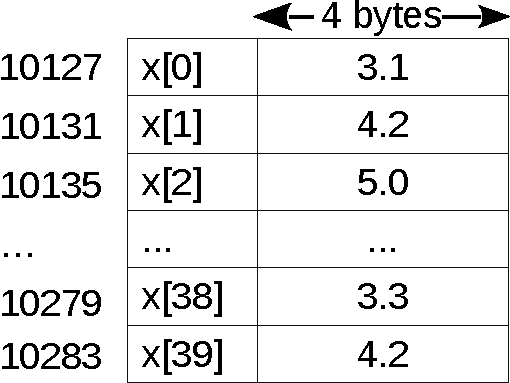
\includegraphics[width=0.90\linewidth]{figs/farray.pdf}
\end{figure}
\end{column}
\begin{column}{0.53\linewidth}
\begin{lstlisting}
#include <stdio.h>
int main()
{
   int a[10], b = 3;
   char c[10];
   printf("a: %d\n", sizeof(a));
   printf("b: %d\n", sizeof(b));
   printf("c: %d\n", sizeof(c));
   return 0;
}
\end{lstlisting}
\end{column}
\end{columns}
\vspace{0.1in}
\begin{itemize}
	\item {The system opens a continuous memory block for an array}
	\item {Actual size depends on both the type and length of an array}
\end{itemize}
\end{frame}

\begin{frame}[fragile]{1D Array: how array looks like (3)}
\begin{columns}
\begin{column}{0.53\linewidth}
\begin{lstlisting}
#include <stdio.h>
int main()
{
   int a[10], b = 3;
   char c[10];
   printf("a: %d\n", sizeof(a));
   printf("b: %d\n", sizeof(b));
   printf("c: %d\n", sizeof(c));
   return 0;
}
\end{lstlisting}
\end{column}
\begin{column}{0.4\linewidth}
[Output]
\begin{lstlisting}
a: 40
b: 4
c: 10
\end{lstlisting}
\end{column}
\end{columns}
\vspace{0.1in}
\begin{itemize}
	\item {Actual size depends on both the type and length of an array}
\end{itemize}
\end{frame}

\begin{frame}[fragile]{1D Array: initialization (1)}
\begin{itemize}
	\item {No initialization, what happens}
\end{itemize}
\vspace{-0.1in}
\begin{columns}
\begin{column}{0.33\linewidth}
[1: local]
\begin{lstlisting}[numbers=none]
#include <stdio.h>
int main()
{
 int a[10];
 int i = 0;
 for(;i < 10; i++)
 printf("%d ",a[i]);
 return 0;
}
\end{lstlisting}
\end{column}
\begin{column}{0.33\linewidth}
[2: static]
\begin{lstlisting}[numbers=none]
#include <stdio.h>
int main()
{
 static int a[10];
 int i = 0;
 for(;i<10; i++)
 printf("%d ",a[i]);
 return 0;
}
\end{lstlisting}
\end{column}
\begin{column}{0.33\linewidth}
[3: external]
\begin{lstlisting}[numbers=none]
#include <stdio.h>
extern a[10];
int main()
{
 int i = 0;
 for(; i<10; i++)
 printf("%d ",a[i]);
 return 0;
}
\end{lstlisting}
\end{column}
\end{columns}
\begin{enumerate}
	\item {Initialize to random numbers}
	\item {Initialize to zeros}
	\item {Initialize to zeros}
\end{enumerate}

\end{frame}

\begin{frame}[fragile]{1D Array: initialization (2)}
\begin{itemize}
	\item {Initializations as follows are \textcolor{green}{valid}}
\end{itemize}
\begin{columns}
\begin{column}{0.45\linewidth}
\begin{lstlisting}
#include <stdio.h>
int main()
{
   int a[10] = {3, 2, 5, 1};
   int i = 0;
   for(; i < 10; i++)
   printf("%d ",a[i]);
   return 0;
}
\end{lstlisting}
\end{column}
\begin{column}{0.45\linewidth}
\begin{lstlisting}
#include <stdio.h>
int main()
{
   int a[] = {3, 2, 5, 1};
   int i = 0;
   for(; i < 4; i++)
   printf("%d ",a[i]);
   return 0;
}
\end{lstlisting}
\end{column}
\end{columns}
\end{frame}

\begin{frame}[fragile]{1D Array: initialization (3)}
\begin{itemize}
	\item {Initializations as follows are \textcolor{red}{invalid}}
\end{itemize}
\begin{columns}
\begin{column}{0.43\linewidth}
\begin{lstlisting}
#include <stdio.h>
int main()
{
   int a[10];
   a[10] = {3, 2, 5, 1};
   int i = 0;
   for(; i < 10; i++)
   printf("%d ",a[i]);
   return 0;
}
\end{lstlisting}
\end{column}
\begin{column}{0.43\linewidth}
\begin{lstlisting}
#include <stdio.h>
int main()
{
   int a = {3, 2, 5, 1};
   int i = 0;
   for(; i < 4; i++)
   printf("%d ",a[i]);
   return 0;
}
\end{lstlisting}
\end{column}
\end{columns}
\end{frame}

\begin{frame}{1D Array Example-1 (1)}
	\begin{itemize}
		\item {Given an array: a[10] = \{3, 21, 5, 8, 5,11, 22,14,9,51\}}
		\item {Flip the array to: \{51, 9, 14, 22, 11, 5, 8, 5, 21, 3\}}
	\end{itemize}
	\vspace{0.2in}
	\begin{center}
		\Large{5 minutes to think about the solution}
	\end{center}
\end{frame}

\begin{frame}{1D Array Example-1 (2)}
	\begin{itemize}
		\item {Given an array: a[10] = \{3, 21, 5, 8, 5,11, 22,14,9,51\}}
		\item {Flip the array to: \{51, 9, 14, 22, 11, 5, 8, 5, 21, 3\}}
	\end{itemize}
	\begin{itemize}
		\item {The idea is that, we only need to swap two elements each time}
		\item {One for the header, one from the rear}
		\item {We do this for $\frac{10}{2}$ times}
	\end{itemize}
\end{frame}

\begin{frame}{1D Array Example-1 (3)}
	\begin{itemize}
		\item {Given an array: a[10] = \{3, 21, 5, 8, 5,11, 22,14,9,51\}}
		\item {Flip the array to: \{51, 9, 14, 22, 11, 5, 8, 5, 21, 3\}}
	\end{itemize}
	\begin{enumerate}
		\item {For i from 0 to $\frac{N}{2}$ do}
		\item {~~~Exchange a[i] with a[N-i-1]}
		\item {End-for}
	\end{enumerate}
	\begin{itemize}
		\item {Let's do it, give you another 5 minutes ...}
	\end{itemize}
\end{frame}

\begin{frame}[fragile]{1D Array Example-1 (4)}
	\begin{enumerate}
		\item {For i from 0 to $\frac{N}{2}$ do}
		\item {~~~Exchange a[i] with a[N-i-1]}
		\item {End-for}
	\end{enumerate}
\begin{lstlisting}[xleftmargin=0.08\linewidth,linewidth=0.9\linewidth]
#include <stdio.h>
int main()
{
   int a[10] ={3,21,5,8,5,11,22,14,9,51};
   int t = 0, i = 0;
   for(; i < 5; i++){
       t = a[i];
       a[i] = a[10-i-1];
       a[10-i-1] = t;
   }
   for(i = 0; i < 10; i++){
       printf("%d ", a[i]);
   }
   return 0;
}
\end{lstlisting}
\end{frame}


\begin{frame}{Dynamic Array Example-2 (1)}
	\begin{itemize}
		\item {An integer number given by user}
		\item {int a[n]}
		\item {Input ``n'' numbers assign to ``a[n]''}
		\item {Print out array ``a''}
	\end{itemize}
	\vspace{0.2in}
	\begin{center}
		\Large{5 minutes to think about the solution}
	\end{center}
\end{frame}

\begin{frame}[fragile]{Dynamic Array Example-2 (2)}
\begin{lstlisting}
#include <stdio.h>
int main()
{
	int n = 0, i = 0;
	scanf("%d", &n);
	int a[n];
	for(i = 0; i < n; i++)
	{
		scanf("%d", &a[i]);
	}
	printf("%d\n", sizeof(a));
	for(i = 0; i < n; i++)
	{
		printf("a[%d] = %d\n", i, a[i]);
	}	
	return 0;
}
\end{lstlisting}

\end{frame}

\begin{frame}{1D Array Example-3 (1)}
	\begin{itemize}
		\item {Given a sorted array: a[7] = \{3, 14, 15, 18, 22,35\}}
		\item {Insert an input number to the array}
		\item {Keep the array sorted after the insertion}
	\end{itemize}
	\vspace{0.2in}
	\begin{center}
		\Large{5 minutes to think about the solution...}
	\end{center}
\end{frame}

\begin{frame}[fragile]{1D Array Example-3 (2)}
\begin{lstlisting}[xleftmargin=0.05\linewidth, linewidth=0.8\linewidth]
#include <stdio.h> 
int main(){
  int a[7] = {3,14,15,18,22,35};
  int b = 7, i = 0, j = 0;
  scanf("%d", &b);
  for(i = 0; i < 6; i++){
    if(b < a[i]){
      break;
	}
  }
  for(j = 6; j > i; j--){
    a[j] = a[j-1];
  }
  a[j] = b;
  for(i = 0; i < 7; i++){
	printf("a[%d] = %d\n", i, a[i]);
  }
  return 0;
}
\end{lstlisting}
\end{frame}

\begin{frame}{1D Array Example-4 (1)}
	\begin{itemize}
		\item {Given an array: a[10] = \{21, 3, 5, 8, 5,11, 22,14,51,9\}}
		\item {Sort the array in ascending order: \{3, 5, 5, 8, 9, 11, 14, 21, 22, 51\}}
	\end{itemize}
	\vspace{0.2in}
	\begin{center}
		\Large{5 minutes to think about the solution...}
	\end{center}
\end{frame}

\begin{frame}{1D Array Example-4 (2)}
	\begin{itemize}
		\item {Given an array: a[10] = \{21, 3, 5, 8, 5,11, 22,14,9,51\}}
		\item {Sort the array in ascending order: \{3, 5, 5, 8, 9, 11, 14, 21, 22, 51\}}
	\end{itemize}
	\begin{itemize}
		\item {The idea is bubble sort, which is a classic method for sorting}
		\item {Each time, we move the largest to the rear of the array}
		\item {Repeat this on sub-array for N times}
	\end{itemize}
\end{frame}

\begin{frame}{1D Array Example-4 (3)}
\begin{figure}
	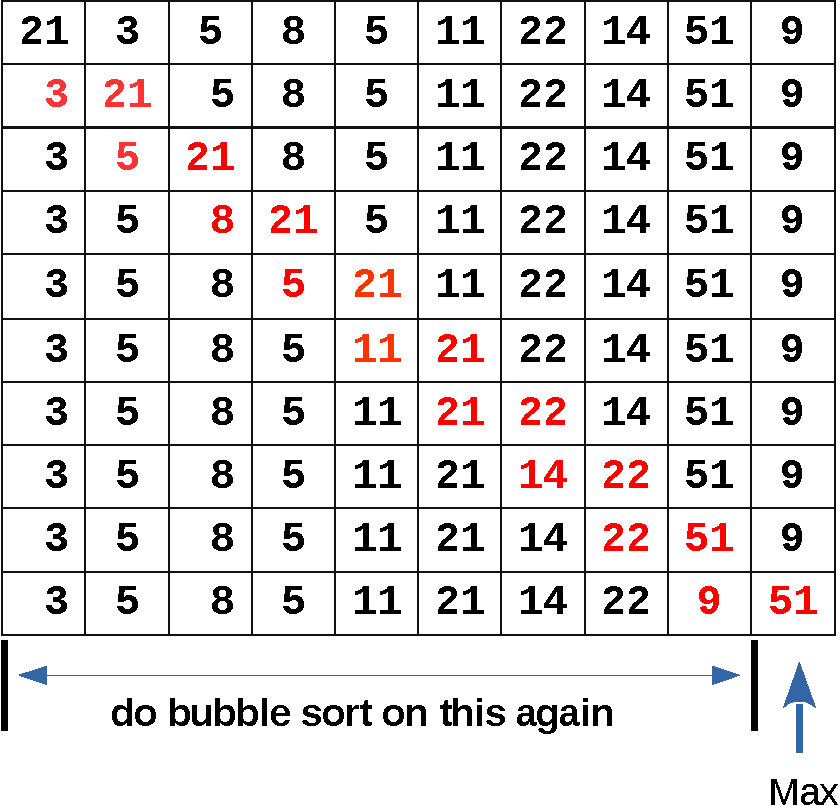
\includegraphics[width=0.55\linewidth]{figs/bubblesort.pdf}
	\caption{Demo of one round of bubble sort}
\end{figure}
\end{frame}

\begin{frame}{1D Array Example-4 (4)}
\begin{itemize}
	\item {Let's now outline the procedure}
\end{itemize}
\begin{enumerate}
	\item {For i from 0 to N do}
	\item {~~For j from 0 to N-i do}
	\item {~~~~Check a[j] and a[j+1]}
	\item {~~~~If a[j] $>$ a[j+1]}
	\item {~~~~~swap them}
	\item {~~~~End-if}
	\item {~~End-for(j)}
	\item {End-for(i)}
\end{enumerate}
\end{frame}

\begin{frame}[fragile]{1D Array Example-4 (5): the code}
\vspace{-0.1in}
\begin{lstlisting}[xleftmargin=0.08\linewidth,linewidth=0.9\linewidth]
#include <stdio.h>
int main()
{
   int a[10] = {3, 5, 5, 8, 9, 11, 14, 21, 22, 51};
   int i = 0, j = 0, t = 0;
   for(i = 0; i < 10; i++) {
      for(j = 0; j < (10-i-1); j++) {
          if(a[j] > a[j+1]) 
          {
             t = a[j];
             a[j] = a[j+1];
             a[j+1] = t;
          }//if(a[j])
      }//for(j)
   }//for(i)
   for(i = 0; i < 10; i++) {
      printf("%d ", a[i]);
   }   
   return 0;
}
\end{lstlisting}
\end{frame}

\subsection{2D Array}
\label{sec:2darry}
\begin{frame}<beamer>
    \frametitle{Outline}
    \tableofcontents[currentsection, currentsubsection]
\end{frame}

\begin{frame}[fragile]{Opening Discussion: 2D Array}
	\begin{itemize}
		\item {Continue with the opening example in the last section}
		\item {In your class, you might have several courses for each student}
		\item {So we need several 1D arrays}
		\item {Alternatively, we can use a 2D array}
	\end{itemize}
\begin{columns}
\begin{column}{0.4\linewidth}
\begin{lstlisting}
int main()
{
    float math[40];
    float c[40];
    float phis[40];
    float bio[40];
    ...
}
\end{lstlisting}
\end{column}
\begin{column}{0.4\linewidth}
\begin{lstlisting}
int main()
{
    float courses[40][4];
    ...
}
\end{lstlisting}
\end{column}
\end{columns}
\end{frame}

\begin{frame}[fragile]{2D Array: declaration}
\begin{center}
	\LARGE{
	 \textcolor{blue}{type} \textcolor{red}{arrayName}[\textbf{row}][\textbf{column}];
	}
\end{center}

	\begin{itemize}
		\item {Similar as 1D array, \textcolor{blue}{type} is required}
		\item {``\textcolor{red}{arrayName}'' should be unique}
		\item {``row'' and ``column'' should be constant expressions}
	\end{itemize}
\begin{lstlisting}
int main()
{
   float a[40][4]; //there 40 rows and 4 columns in each row
   a[3][2] = 3.14;
   return 0;
}
\end{lstlisting}
\end{frame}

\begin{frame}[fragile]{2D Array: initialization (1)}
\begin{lstlisting}
int main()
{
   float a[3][4] = {{1,3,1,1},{1,2,1,3},{1,12,1,2}};
   return 0;
}
\end{lstlisting}
\begin{itemize}
	\item {Following way is also \textcolor{green}{valid}}
\end{itemize}
\begin{lstlisting}
int main()
{
   float a[3][4] = {1,3,1,1,1,2,1,3,1,12,1,2};
   return 0;
}
\end{lstlisting}
\end{frame}

\begin{frame}[fragile]{2D Array: initialization (2)}
\begin{lstlisting}
int main()
{
   float a[][4] = {{1,3,1,1},{1,2,1,3},{1,12,1,2}};
   return 0;
}
\end{lstlisting}
\begin{itemize}
	\item {Following way is also \textcolor{green}{valid}, $row=\lceil\frac{N}{4}\rceil$}
\end{itemize}
\begin{lstlisting}
int main()
{
   float a[][4] = {1,3,1,1,1,2,1,3,1,12,1,2};
   return 0;
}
\end{lstlisting}
\begin{itemize}
	\item {If no initialization, set to \textcolor{red}{0} by default}
\end{itemize}
\end{frame}

\begin{frame}[fragile]{2D Array: initialization (3)}
\begin{lstlisting}
int main()
{
   float a[][4] = {{1,3,1,1},{1,2,1,3},{1,12,1,2}};
   return 0;
}
\end{lstlisting}
\begin{itemize}
	\item {Following way is also \textcolor{red}{invalid}}
\end{itemize}
\begin{lstlisting}
int main()
{
   float a[4][] = {1,3,1,1,1,2,1,3,1,12,1,2};
   return 0;
}
\end{lstlisting}
\begin{itemize}
	\item {It is organized in row major order}
\end{itemize}
\end{frame}

\begin{frame}[fragile]{2D Array: how it looks like}
\begin{figure}
	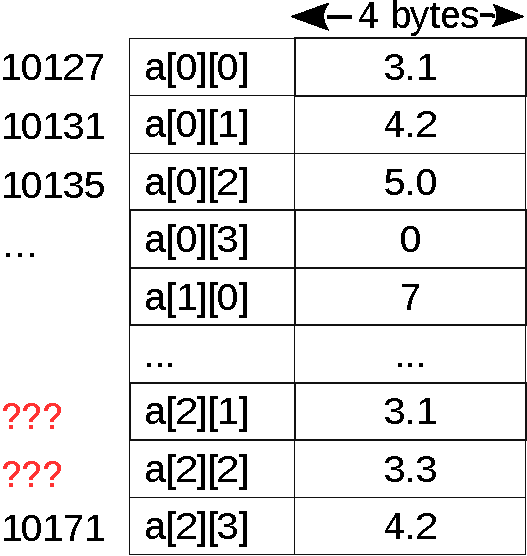
\includegraphics[width=0.4\linewidth]{figs/farray2d.pdf}
\end{figure}
\begin{itemize}
	\item {$3$(row)${\times}4$(column)${\times}4$ bytes}
\end{itemize}
\end{frame}

\begin{frame}[fragile]{2D Array: visit element of the array}
\begin{lstlisting}[xleftmargin=0.08\linewidth, linewidth=0.85\linewidth]
int main()
{
   float a[][4] = {1,3,1,1,1,2,1,3,1,12,1,2};
   int i = 0, j = 0;
   for(i = 0; i < 3; i++)
   {
      for(j = 0; j < 4; j++)
      {
          printf("%f ", a[i][j]);
      }
      printf("\n");
   }
   return 0;
}
\end{lstlisting}
\end{frame}


\begin{frame}{Example-1: transpose a matrix (1)}
\begin{itemize}
	\item {Given a 2D matrix, kept in a 1D array}
	\item {a[12] = \{12,13,5,5,7,21,6,4,10,5,5,9\}}
\end{itemize}
\vspace{-0.1in}
\begin{columns}
\begin{column}{0.4\linewidth}
\begin{equation}
A=\left[
\begin{array}{ccc}
12 & 13 & 5 \\
5 & 7 & 21 \\
6 & 4 & 10 \\
5 & 5 & 9 
\end{array}
\right]_{3{\times}4} \nonumber
\end{equation}
\end{column}
\begin{column}{0.1\linewidth}
\begin{center}
$\Rightarrow$
\end{center}
\end{column}
\begin{column}{0.4\linewidth}
\begin{equation}
A^T=\left[ 
\begin{array}{cccc}
12 & 5 & 6 & 5 \\
13 & 7 & 4 & 5 \\
5 & 21 & 10 & 9
\end{array}
\right]_{4{\times}3} \nonumber
\end{equation}
\end{column}
\end{columns}
\begin{itemize}
	\item {a[12] =\{12,5,6,5,13,7,4,5,5,21,10,9\}}
\end{itemize}
\begin{enumerate}
	\item {A[i][j] $\rightleftarrows$ A[j][i]}
	\item {A[i][j] $\Rightarrow$ a[i*c1+j]}
	\item {A[j][i] $\Rightarrow$ b[j*c2+i]}
	\item {a[i*c1+j] $\rightleftharpoons$ b[j*c2+i]}
\end{enumerate}
\end{frame}

\begin{frame}[fragile]{Example-1: transpose a matrix (2)}
\begin{lstlisting}[xleftmargin=0.08\linewidth, linewidth=0.85\linewidth]
#include <stdio.h>
int main(){
  int a[12] = {12,13,5,5,7,21,6,4,10,5,5,9};
  int b[12] = {0};
  int i = 0, j = 0, tmp = 0;
  for(i = 0; i < 4; i++){
    for(j = 0; j < 3; j++){
      b[j*4+i] = a[i*3+j];
    }
  }
  for(i = 0; i < 3; i++){
    for(j = 0; j < 4; j++){
       printf("%4d", b[i*4+j]);
    }
    printf("\n");
  }
  return 0;
}
\end{lstlisting}
\end{frame}
